\chapter{Polynomial Eigenvalue Problem} \label{chap:polynomial-eigenvalue-problem}
Magnetic field lines guide the motion of charged particles in plasma. In this chapter, we first examine the single particle motion along the magnetic field, subsequently to a kinetic description of plasma. Following this, we derive the fluid description of plasma using the fact that fluid velocity follows the magnetic field line $\mathbf{v} = v\mathbf{B}/B$. After this, we establish the governing equations for flow in the magnetic nozzle. Following their derivation, we proceed to linearize these governing equations and reframe the problem as a polynomial eigenvalue problem. Finally, we analytically explore a special case.

\section{Kinetic Theory}
\subsection{Single Particle Motion in Uniform Magnetic and Electric Fields} \label{sec:single-particle-motion}
Plasma consists of charged particles, and is governed by electromagnetic force. This subsection gives a description of single particle motion with the presence of uniform magnetic and electric fields. This gives us intuition of how the particles move in a magnetic nozzle. Since the particle motion is governed by Lorentz force, the equation of motion of a charged particle is given by
\begin{equation}
	m\dv{\mathbf{v}_p}{t} = q(\mathbf{E} + \mathbf{v}_p\times \mathbf{B})
	\label{eq:equation-of-motion-single-particle}
\end{equation}
where $m$ is the mass of charged particle, $q$ is its electric charge, and $\mathbf{v}_p$ is the particle's velocity.

\subsubsection*{No Electric Field}
Consider a uniform magnetic field pointing in z-direction, $\mathbf{B}=B\mathbf{\hat{z}}$, and no electric field for now. Since the magnetic force is perpendicular to both $\mathbf{v}_p$ and $\mathbf{B}$, we can separate the equation of motion into two directions,
\begin{equation}
	\begin{aligned}
		m\dv{\mathbf{v_\parallel}}{t} & = \mathbf{0}                 \\
		m\dv{\mathbf{v_\perp}}{t}     & = q\mathbf{v_\perp \times B}
	\end{aligned}
\end{equation}
where $\mathbf{v_\parallel}$ denotes the velocity along the magnetic field line, in this case $v_\parallel = v_z$, and $\mathbf{v_\perp}$ is the velocity perpendicular to the magnetic field, in this case $\mathbf{v_\perp} = v_x\hat{x} + v_y\hat{y}$. Solving these equations with initial condition $\mathbf{v_p}|_{t=0} = v_{0x}\hat{x} + v_{0y}\hat{y} + v_{0z}\hat{z}$  we get
\begin{equation}
	\begin{aligned}
		v_x & = v_{0\perp} e^{i\omega_c t}      \\
		v_y & = \pm iv_{0\perp} e^{i\omega_c t} \\
		v_z & = v_{0z}
	\end{aligned}
\end{equation}
where $v_{0\perp} = \sqrt{v_{0x}^2+v_{0y}^2}$ is the initial speed in the plane perpendicular to the magnetic field, and $\omega_c \equiv \abs{q}B/m$ is called the Larmor frequency. In this way, we see that the charged particle is doing circular motion in the $x-y$ plane with Larmor frequency $\omega_c$. On the other hand, the particle is flowing freely in $\hat{z}$ direction since there is no force acting on the charged particle along the magnetic field line. The charged particle is doing helical motion along the magnetic field line. See Fig.~\ref{fig:gyrate-along-b-field}. If we integrate the velocities with respect to time we will see the radius of the gyration is a constant, $r_L \equiv m_v\perp/\abs{q}B$, it is called Larmor radius.

\subsubsection*{Finite Electric Field}
With the presence of uniform electric field $\mathbf{E} = E_x\hat{x} + E_y\hat{y} + E_z\hat{z}$, the solution to Eq.~(\ref{eq:equation-of-motion-single-particle}) becomes

\begin{equation}
	\begin{aligned}
		v_x & = v_{0\perp} e^{i\omega_c t} + \frac{E_y}{B}      \\
		v_y & = \pm iv_{0\perp} e^{i\omega_c t} - \frac{E_x}{B} \\
		v_z & = v_{0z} + \frac{qE_z}{m}t
	\end{aligned}
\end{equation}
In the direction along the magnetic field, electrostatic force is acting on the particle causing it to accelerate / decelerate with constant acceleration $qE_z/m$. In the direction perpendicular to magnetic field, the Larmor radius is still $r_L = m_v\perp/\abs{q}B$ but the particle's guiding center drifts with velocity
\begin{equation}
	\mathbf{v_{E\times B}} = \frac{\mathbf{E\times B}}{B^2} = \frac{E_y}{B}\hat{x} - \frac{E_x}{B}\hat{y}
\end{equation}
This is so-called the $\mathbf{E\times B}$ drift.

Imagine a cylinder shape magnetic nozzle with externally applied magnetic field, the magnetic field is as described in Sec.~\ref{sec:magnetic-field-in-nozzle}. The particles will move along the magnetic field lines. Due to high mobility of electrons, they move faster than ions, this creates electric field and will accelerate ions in the nozzle (more details will be discussed in Sec.~\ref{sec:equation-of-motion-of-the-plasma-flow-in-nozzle}). By symmetry, if there is electric field in the plane perpendicular to $\mathbf{B}$ field, it will be pointing radially, $\mathbf{E_\perp} = E_\perp\cos\theta\hat{x} + E_\perp\sin\theta\hat{y}$. According to the above discussion, the $\mathbf{E\times B}$ drift, $\mathbf{v_{E\times B}} = E_\perp/B (\sin\theta\hat{x} - \cos\theta\hat{y})$, will be in $\hat{\theta}$ direction. Meaning that in magnetic nozzle, the particles have two gyrating motions: one is the small scale Larmor gyration, and the other one is the larger scale $\mathbf{E\times B}$ drift in $\hat{\theta}$ direction. In this thesis, we are interested in the flow near the central axis, therefore the larger scale drift will be ignored.

\subsection{Adiabatic Invariants}
The charged particles always travel on the same magnetic field line in the magnetic nozzle. To show this we will introduce two adiabatic invariants.

\subsubsection*{Magnetic Moment}
In classical mechanics, the action integral $\oint pdq$ taken over a period of a periodic motion is a constant. Here $p$ and $q$ are generalized momentum and coordinate. In single particle motion along magnetic field line, one obvious periodic motion is the Larmor gyration. Take $p$ to be the angular momentum $mv_\perp r$ and $q$ to be the angular coordinate $\theta$, the action integral becomes

\begin{equation}
	\oint pdq = \oint mv_\perp r_L d\theta = 2\pi r_L mv_\perp = 2\pi \frac{mv_\perp^2}{\omega_c} = 4\pi\frac{m}{\abs{q}}\left(\frac{mv_\perp^2}{2B}\right)
\end{equation}

Define the quantity magnetic moment as

\begin{equation}
	\mu = \frac{mv_\perp^2}{2B}
\end{equation}

We see that the magnetic moment $\mu$ is constant as long as $q/m$ is constant.

\subsubsection*{Longitudinal Invariant}
The next adiabatic invariant is the quantity defined as \cite{chen_introduction_2016},
\begin{equation}
	J=\int_a^b v_\parallel ds
\end{equation}
where $a$ and $b$ are the two turning points in magnetic mirror, see Fig.~\ref{fig:particle-in-mirror}.

\begin{figure}[htbp]
	\centering
	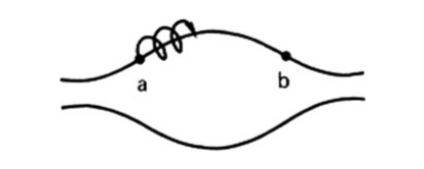
\includegraphics[width=0.4\textwidth]{figures/particle-in-mirror.tikz}
	\caption{A particle bouncing between turning points $a$ and $b$ in a magnetic field. Adapted from \cite{chen_introduction_2016}.}
	\label{fig:particle-in-mirror}
\end{figure}

Since the particle's energy is conserved and is equal to $mv_\perp^2/2$ at the turning point, the invariance of $\mu$ indicates that $\abs{B}$ remains the same at the turning point. However, upon drifting back to the same longitude, a particle may find itself on another line of force at a different altitude. This cannot happen if $J$ is conserved. $J$ determines the length of the line of force between turning points, and no two lines have the same length between points with the same $\abs{B}$. Consequently, the particle returns to the same line of force even in a slightly asymmetric field.


\begin{figure}[htbp]
	\centering
	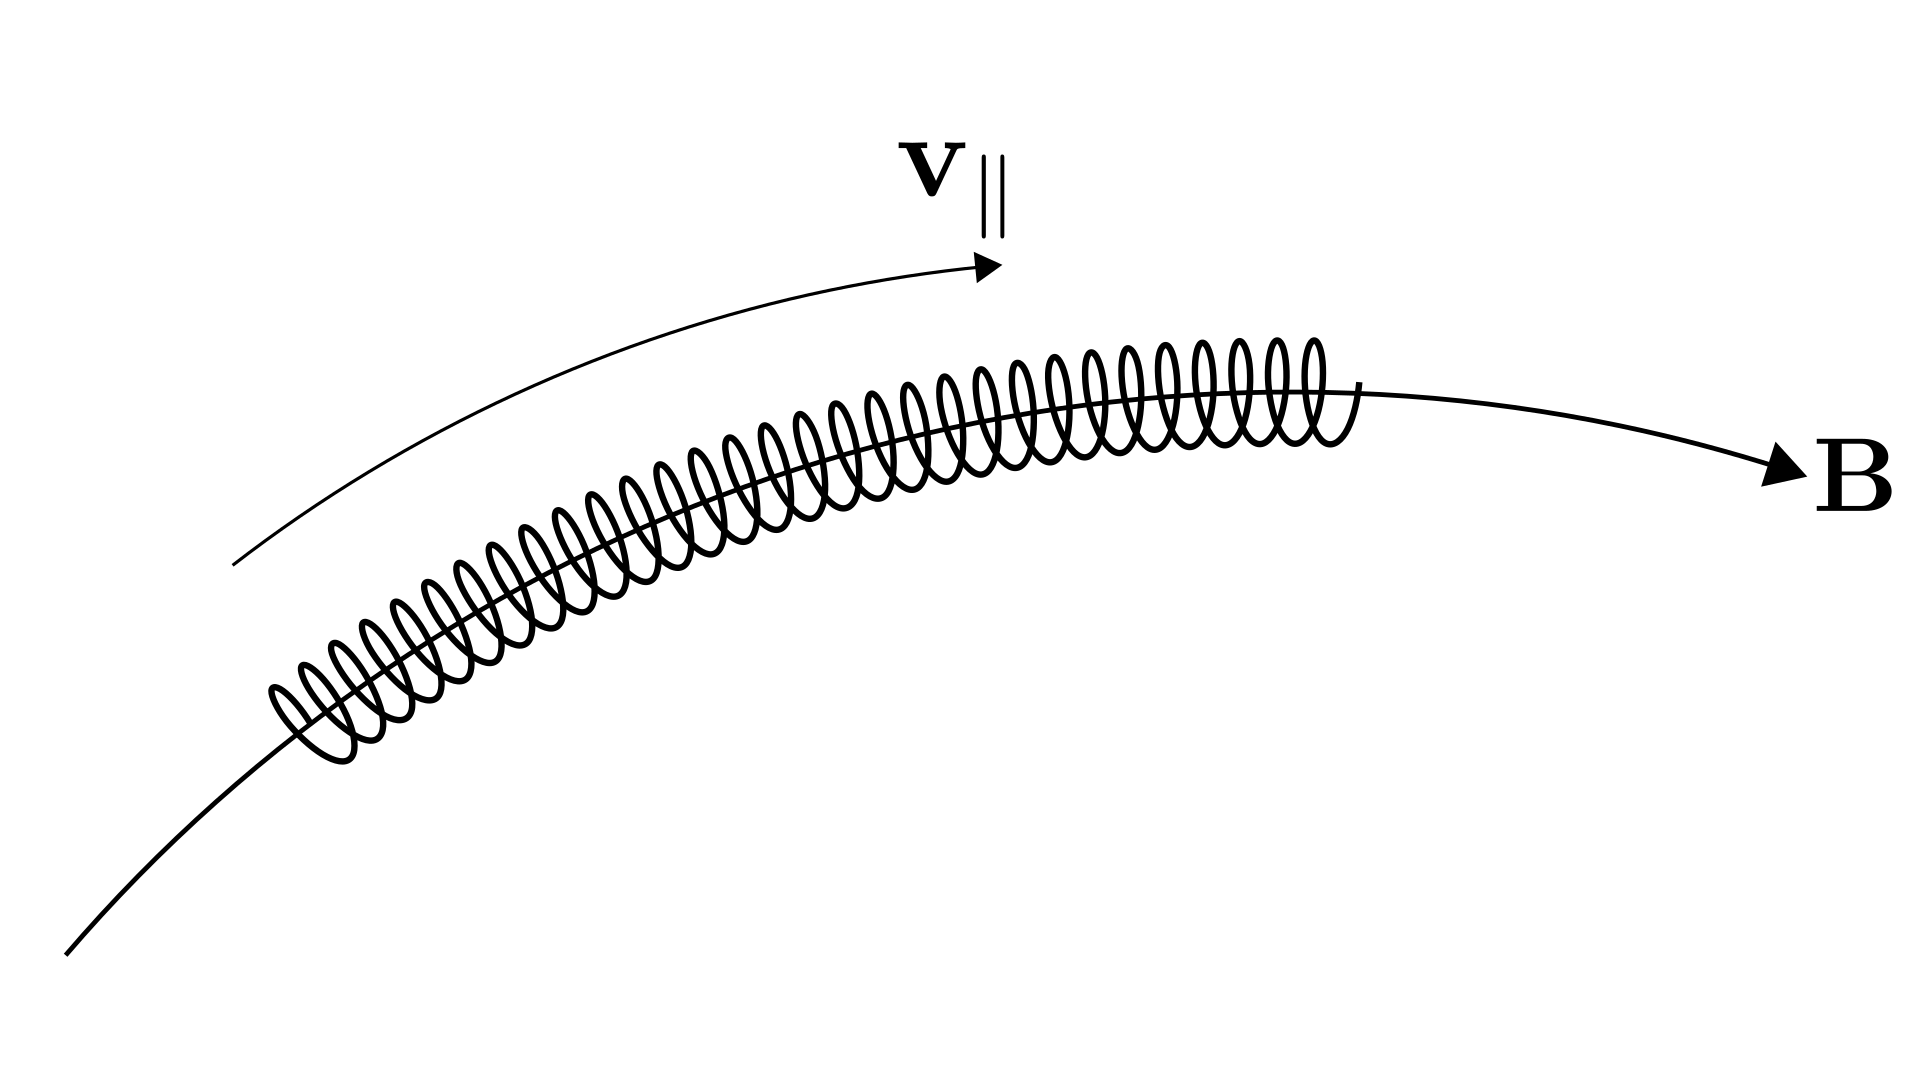
\includegraphics[width=0.7\linewidth]{figures/gyrate-along-b-field}
	\caption{A charged particle gyrates about the magnetic field line. The velocity along the field line is $\mathbf{v}_{\parallel}$ and the gyrate frequency, radius is given by the radial equation, $q\mathbf{v_{\perp}\times B} = \mathbf{\hat{r}} mv_\perp^2/r$. Moreover, for static, nonuniform magnetic field, the charged particle will stay on the same of magnetic field line as it gyrates.}
	\label{fig:gyrate-along-b-field}
\end{figure}

\subsection{From Kinetic Theory to Fluid Description}
Although the previous treatment is useful for single particle, to describe the collective behavior of a large amount of particles, we need to do that in the framework of kinetic theory. In kinetic theory, the charged particles in plasma obey a certain velocity distribution function,
\begin{equation}
	f(\mathbf{x}, \mathbf{v}_p, t)
\end{equation}
The number of particles per m$^3$ at position $\mathbf{x}$ and time $t$ with velocity components in the cell bounded by $\mathbf{v}$ and $\mathbf{v}+d\mathbf{v}$ is
\begin{equation}
	f(\mathbf{x}, \mathbf{v}_p, t)d^3\mathbf{v}_p
\end{equation}

Suppose a collisionless plasma in 3-dimensional space is at thermal equilibrium, then the particles can be characterized by Maxwell-Boltzmann distribution
\[ f_M(\mathbf{x}, \mathbf{v}_p, t) = \frac{n(\mathbf{x}, t)}{(\pi v_{th}^2)^{3/2}} \exp(-\left(\frac{v}{v_{th}}\right)^2) \]
where $n(\mathbf{x},t)$ is number density of the particles, $v_{th} = \sqrt{2k_BT/m}$ is the thermal velocity, and $v=\sqrt{v_x^2+v_y^2+v_z^2}$.

The moments of the distribution function are suitable macroscopic properties of the plasma. For example, the plasma number density and momentum can be viewed as

\begin{equation}
	\begin{aligned}
		n(\mathbf{x}, t)           & = \int_{\mathbb{R}^3} f(\mathbf{x}, \mathbf{v}_p, t) d^3\mathbf{v}_p              \\
		n\mathbf{v}(\mathbf{x}, t) & = \int_{\mathbb{R}^3} \mathbf{v}_p f(\mathbf{x}, \mathbf{v}_p, t) d^3\mathbf{v}_p
	\end{aligned}
\end{equation}
where $\mathbf{v}$ without the subscript $p$ is the fluid velocity of the plasma flow. It is the bulk velocity of the plasma. The charged particles flow along the magnetic field line, it is intuitive to think of $\mathbf{v}$ as the plasma flow velocity along the magnetic field line.

In this thesis we assume collisionless plasma. The distribution function $f$ in a collisionless plasma satisfies the so-called collisionless Vlasov equation, $\dv*{t} f(\mathbf{x}, \mathbf{v}, t) = 0$. Expand it explicitly, it is
\begin{equation} \label{eq:vlasov}
	\pdv{f}{t} + \mathbf{v}\pdv{f}{\mathbf{x}} + \frac{q}{m}(\mathbf{E} + \mathbf{v}\times\mathbf{B})\pdv{f}{\mathbf{v}} = 0
\end{equation}
where $q(\mathbf{E} + \mathbf{v}\times\mathbf{B})$ is the Lorentz force experience by the species, the collision term $C(f)$ is dropped.

Integrate both sides with respect to volume element in velocity space, $d^3\mathbf{v}$, we get the conservation of density.
\begin{equation}
	\pdv{n}{t} + \div(n\mathbf{v}) = 0
\end{equation}

If we multiply $\mathbf{v}$ on both sides and integrate with respect to $d^3\mathbf{v}$, we get the conservation of momentum.
\begin{equation}
	mn\left[\pdv{\mathbf{v}}{t} + (\mathbf{v}\cdot\grad){\mathbf{v}} \right] = qn(\mathbf{E+v\times B}) - \div\mathbf{P} + \mathbf{P}_{ij}
\end{equation}
where $\mathbf{P}\equiv mn\overline{\mathbf{v}}_{thermal}\overline{\mathbf{v}}_{thermal}$, the bar represents average over velocity space with distribution function $f(\mathbf{x}, \mathbf{v}_p, t)$, is the stress tensor. If we assume isothermal plasma with isotropic pressure, $p=nKT$ where $T$ is constant, then the last two terms can be simplified to $\grad p = KT\grad n$.

As we can see the fluid description only depends on the macroscopic properties of plasma, such as the fluid velocity along the magnetic field line $\mathbf{v}$, number density $n$, and pressure $p$ of the plasma. This simplifies the problem.

\section{Equation of Motion of the Plasma Flow in Nozzle} \label{sec:equation-of-motion-of-the-plasma-flow-in-nozzle}
In this section, we will derive the governing equations of the quasineutral plasma flow with cold magnetic ions in magnetic nozzle under paraxial approximation.

Starting from the conservation of number density,
\begin{equation}
	\pdv{n}{t} + \div(n\mathbf{v}) = 0
\end{equation}
Since ions carry most of the mass and momentum in the plasma, their velocity is more representative of the bulk flow of the plasma. Electrons, on the other hand, have much smaller mass and are highly mobile due to their low inertia, but they contribute less to the overall momentum of the flow. As we discussed in the Sec.~\ref{sec:single-particle-motion}, the charged particles are doing helical motions along the magnetic field lines. Hence, we take the fluid velocity as the ion velocity along the magnetic field lines
\begin{equation}
	\mathbf{v} = v\mathbf{B}/B
\end{equation}
By expanding the divergence term $\div(n\mathbf{v})$, and using the divergence free condition $\div B=0$, we have
\begin{equation}
	\pdv{n}{t} + \mathbf{B}\cdot \grad(\frac{nv}{B}) = 0
\end{equation}
Using the paraxial approximation, $\grad_\parallel = \partial_z\hat{z}$. We obtain the conservation of density for the magnetic nozzle,
\begin{equation}
	\pdv{n}{t} + B\pdv{z}(\frac{nv}{B}) = 0
\end{equation}

The conservation of momentum for ions and electrons are
\begin{align}
	 & m_in\left[\pdv{\mathbf{v}}{t} + (\mathbf{v}\cdot\grad)\mathbf{v}\right] = en(\mathbf{E}+\mathbf{v}\times\mathbf{B})                \\
	 & m_en\left[\pdv{\mathbf{v}}{t} + (\mathbf{v}\cdot\grad)\mathbf{v}\right]  = -en(\mathbf{E}+\mathbf{v}\times\mathbf{B}) - \grad{p_e}
\end{align}
where $p_e$ is the electron pressure. There are some simplifications, first is that the term $\mathbf{v\times B} = 0$ due to the fact that fluid velocity is along $\mathbf{B}$. Secondly, $m_en\dv{\mathbf{v}}{t} \simeq 0$ due to small electron mass. Hence, the above two equations becomes,
\begin{align}
	 & m_in\left[\pdv{v}{t} + v\pdv{v}{z}\right] = enE_\parallel \\
	 & 0 = -enE_\parallel - \pdv{p_e}{z}
\end{align}
Adding these two equations we obtain
\begin{equation}
	\pdv{v}{t} + v\pdv{v}{z} = -\frac{1}{m_in}\pdv{p_e}{z}
\end{equation}

Assume isothermal, then the electron pressure, also called the equation of state, is
\begin{equation} \label{eq:eos}
	p_e = nKT_e
\end{equation}
We can make this assumption due to the fact the electrons are so mobile that their heat conductivity is almost infinite \cite{chen_introduction_2016}.

Therefore, we have
\begin{equation}
	\pdv{v}{t} + v\pdv{v}{z} = -c_s^2\frac{1}{n}\pdv{n}{z}
\end{equation}
where $c_s^2 = KT_e/m_i$ is the square of ion sound speed.

Therefore, the dynamics of the plasma flow in magnetic nozzle can be characterized by the conservation of density and momentum,
\begin{align*}
	 & \pdv{n}{t} + B\pdv{z}(\frac{nv}{B}) = 0                \\
	 & \pdv{v}{t} + v\pdv{v}{z} = -c_s^2\frac{1}{n}\pdv{n}{z}
\end{align*}
The magnetic field profile was discussed in Sec.\ref{sec:magnetic-field-in-nozzle}.

From the above derivation, it is clear that due to finite temperature and high mobility of the electrons, they establish the electric field to accelerate the cold magnetized ions in the nozzle. The thermal energy of the electrons are converted to kinetic energy of ions in this setup.

For convenience, we nondimensionalize the governing equations by normalizing the velocity to $c_s$, $v\mapsto v/c_s$, $z$ to system length $L$, $z \mapsto z/L$ and time $t\mapsto c_s t/L$. The governing equations become
\begin{align}
	 & \pdv{n}{t} + n\pdv{v}{z} + v\pdv{n}{z} - nv\frac{\partial_z B}{B} = 0
	\label{eq:conservation-of-density}
	\\
	 & n\pdv{v}{t} + nv\pdv{v}{z} = -\pdv{n}{z}
	\label{eq:conservation-of-momentum}
\end{align}
In the later thesis, we will refer the governing equations to Eq.~(\ref{eq:conservation-of-density}), (\ref{eq:conservation-of-momentum}) without mentioning the nondimensionalization.

\section{Velocity Profiles at Equilibrium}
\subsection{Lambert $W$ Function}
Lambert $W$ function is necessary for the following discussion.
\begin{definition}
	The Lambert $W$ function is a function, $y(x)$, such that $ye^y = x$ holds, where $x,y\in\mathbb{R}$.
\end{definition}
It is denoted as $W_k(x)$, where $k = 0,-1$ are its two branches. See Fig.~\ref{fig:lambert-w}.
\begin{figure} [htbp]
	\centering
	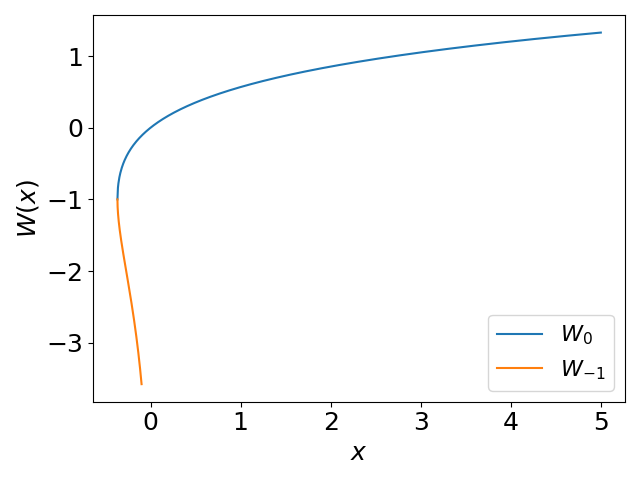
\includegraphics[width=0.6\textwidth]{figures/lambert-w.png}
	\caption{The graph of $y=W(x)$ for real $x<5$ and $y>-4$. The upper branch (blue) with $y\geq-1$ is the graph of the function $W_0(x)$ (principal branch), the lower branch (orange) with $y\leq -1$ is the graph of the function $W_{-1}(x)$. The left most point of the curve is at $(-1/e,-1)$.}
	\label{fig:lambert-w}
\end{figure}

\subsection{Velocity Profiles}
In this research, we are interested in the stability of such plasma flow in the nozzle at equilibrium. Let's denote $n_0$ and $v_0$ as equilibrium density and equilibrium velocity, respectively. Since they are stationary (time independent) solutions to the governing equations Eq.~(\ref{eq:conservation-of-density}), (\ref{eq:conservation-of-momentum}), they satisfy the so-called equilibrium condition (nondimensionalized),
\begin{align}
	 & \pdv{z}(\frac{n_0v_0}{B}) = 0 \label{eq:equilibrium-conservation-of-density}                 \\
	 & v_0\pdv{v_0}{z} = -\frac{1}{n_0}\pdv{n_0}{z} \label{eq:equilibrium-conservation-of-momentum}
\end{align}

In this section we will solve the equilibrium velocity profile, $v_0$, from the nondimensionalized equilibrium condition, Eq.~(\ref{eq:equilibrium-conservation-of-density}) and Eq.~(\ref{eq:equilibrium-conservation-of-momentum}).
We start by substituting $\frac{1}{n_0}\pdv*{n_0}{z}$ into Eq.~(\ref{eq:equilibrium-conservation-of-density}), then it becomes
\begin{equation}
	(v_0^2-1)\pdv{v_0}{z} = -\frac{v_0}{B}\pdv{B}{z}
\end{equation}

Notice that there is a singularity at $v_0=1$, the sonic speed. Later we will devote an entire Chap.~\ref{chap:singular-perturbation} to discuss the treatment for solving eigenvalues involving this singularity.

We can solve the equation by separating the variables, i.e. $v_0$ on one side and $B$ on the other side of the equal sign. Then integrate equation with respect to $z$ and use the conditions at midpoint $B(0)=B_m, v_0(0)=v_m$ we get
\begin{equation}
	v_0^2e^{-v_0^2} = \frac{B^2}{B_m^2}v_m^2e^{-v_m^2}
\end{equation}
We can now express $v_0$ using the Lambert W function,
\begin{equation}
	v_0(z) = \left[ -W_k\left(-\frac{B(z)^2}{B_m^2}v_m^2e^{-v_m^2}\right) \right]^{1/2}
	\label{eq:velocity-profile}
\end{equation}
where the subscript $k$ of $W$ stands for branch of Lambert W function.

When considering the velocity profile of a nozzle flow, various scenarios can be distinguished based on the Mach number parameter ($v_m$) and the branch ($k$) used in the expression for the Mach number distribution, denoted as $v_0(z)$. These parameters play a crucial role in determining the flow characteristics. The selection of appropriate $v_m$ and $k$ values facilitates the control of the flow characteristics in the nozzle, allowing for the realization of various flow regimes, such as subsonic, supersonic, transonic, accelerating, or decelerating profiles. Different velocity profiles are shown in Fig.~\ref{fig:velocity-profiles}.
\begin{itemize}
	\item Subsonic profile: when $v_m < 1$ and $k = 0$, the resulting velocity profile is classified as subsonic. This means that both at the entrance and exit of the nozzle, the velocity remains subsonic, and the midpoint velocity is also less than unity ($v_m < 1$). A subsonic flow is characterized by fluid velocities that are slower than the local speed of sound. The blue and orange curves on Fig.~\ref{fig:velocity-profiles} are both subsonic profiles. As $z$ goes from $-1$ to $0$, the point $(z,W)$ moves towards the point $(-1/e, 1)$ along the $k=-1$ branch. As $z$ goes from $0$ to $1$, the point $(z, W)$ moves away $(-1/e,1)$ along the same $k=-1$ branch.
	\item Supersonic profile: when $v_m > 1$ and $k = -1$, the velocity profile corresponds to a supersonic flow. In this situation, the fluid velocities at both the entrance and exit of the nozzle are supersonic, and the midpoint velocity ($v_m$) exceeds the value of unity ($v_m > 1$). Supersonic flow is characterized by velocities that surpass the speed of sound. The purple and brown curves on Fig.~\ref{fig:velocity-profiles} are both supersonic profiles. As $z$ goes from $-1$ to $0$, the point $(z,W)$ moves towards the point $(-1/e, 1)$ along the $k=0$ branch. As $z$ goes from $0$ to $1$, the point $(z, W)$ moves away $(-1/e,1)$ along the same $k=0$ branch.
	\item Accelerating profile: when $v_m = 1$, the velocity profile becomes transonic. In this case, the midpoint velocity is exactly at the sonic threshold ($v_m = 1$), where the fluid velocity equals the local speed of sound. To achieve an accelerating velocity profile, a configuration with $k = 0$ for $z < 0$ and $k = -1$ for $z > 0$ is employed. Here, $z$ represents the spatial coordinate along the nozzle length. With this setup, the flow starts subsonically and gradually accelerates to a supersonic speed as it propagates along the nozzle. The green curve on Fig.~\ref{fig:velocity-profiles} is the accelerating profile. As $z$ goes from $-1$ to $0$, the point $(z,W)$ moves towards the point $(-1/e, 1)$ along the $k=-1$ branch. As $z$ goes from $0$ to $1$, the point $(z, W)$ moves away $(-1/e,1)$ along another branch, $k=0$.
	\item Decelerating profile: set $v_m = 1$ again, then a decelerating velocity profile can be obtained by adopting a similar approach but with reversed values of $k$. Specifically, the configuration will have $k = -1$ for $z < 0$ and $k = 0$ for $z > 0$, causing the flow to start supersonically and decelerate to subsonic velocities further down the nozzle. The red curve on Fig.~\ref{fig:velocity-profiles} is the decelerating profile. As $z$ goes from $-1$ to $0$, the point $(z,W)$ moves towards the point $(-1/e, 1)$ along the $k=0$ branch. As $z$ goes from $0$ to $1$, the point $(z, W)$ moves away $(-1/e,1)$ along another branch, $k=-1$.
\end{itemize}


\begin{figure}[htbp]
	\centering
	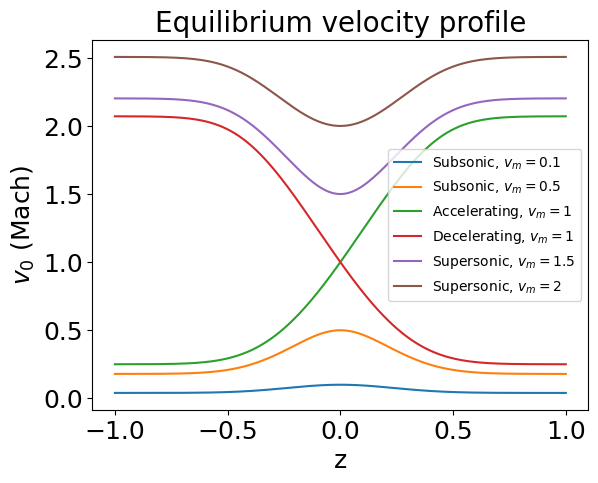
\includegraphics[width=0.7\linewidth]{figures/velocity-profiles}
	\caption{The velocity profile in the magnetic nozzle is completely determined by the midpoint mach number $v_m$ and the branch $k$. A subsonic profile can be obtained by selecting $v_m<1$ and $k=0$. On the other hand, a supersonic profile can be obtained by setting $v_m>1$ and $k=-1$. Lastly, for the transonic velocity profiles, the midpoint velocity is set to unity, $v_m=1$, and then by choose $k=0$ for $x<0$ and $k=-1$ for $x>0$ we get accelerating profile. Decelerating profile can be obtained similarly.}
	\label{fig:velocity-profiles}
\end{figure}

\section{Linearized Governing Equations}
As illustrated in Sec.\ref{sec:instability-of-plasma-flow}, it is essential to linearize the governing equations in order to investigate the linear instability of plasma. Now we are going to derive the linearized governing equations with the equilibrium conditions given in above.

Let $n = n_0(z) + \tilde{n}(z,t)$ and $v = v_0(z) + \tilde{v}(z,t)$, where $\tilde{n}$ and $\tilde{v}$ are small perturbed quantities.

We first linearize Eq.~(\ref{eq:conservation-of-density}) by setting $n=n_0+\tilde{n}$ and $v=v_0+\tilde{v}$,
\[    \pdv{(n_0+\tilde{n})}{t}
	+ (n_0+\tilde{n})\pdv{(v_0+\tilde{v})}{z}
	+ (v_0+\tilde{v})\pdv{(n_0+\tilde{n})}{z}
	- (n_0+\tilde{n})(v_0+\tilde{v})\frac{\partial_z B}{B} = 0
\]
By ignoring the nonlinear terms, we obtain
\[ \frac{1}{n_0}\pdv{\tilde{n}}{t}
	+ \pdv{v_0}{z} + \frac{\tilde{n}}{n_0}\pdv{v_0}{z} + \pdv{\tilde{v}}{z}
	+ \frac{v_0}{n_0}\pdv{n_0}{z} + \frac{\tilde{v}}{n_0}\pdv{n_0}{z} + \frac{v_0}{n_0}\pdv{\tilde{n}}{z}
	- v_0\frac{\partial_z B}{B} - \tilde{v}\frac{\partial_z B}{B} - \tilde{n}\frac{v_0}{n_0}\frac{\partial_z B}{B} = 0
\]

Using the equilibrium condition Eq.~(\ref{eq:equilibrium-conservation-of-density}), $\partial_zv_0+v_0\partial_zn_0/n_0$ cancels $-v_0\partial_zB/B$,
\[ \frac{1}{n_0}\pdv{\tilde{n}}{t}
	+ \frac{\tilde{n}}{n_0}\pdv{v_0}{z} + \pdv{\tilde{v}}{z}
	+ \frac{\tilde{v}}{n_0}\pdv{n_0}{z} + \frac{v_0}{n_0}\pdv{\tilde{n}}{z}
	- \tilde{v}\frac{\partial_z B}{B} - \tilde{n}\frac{v_0}{n_0}\frac{\partial_z B}{B} = 0
\]

Moreover, the last term can be written as
\[ \tilde{n}\frac{v_0}{n_0}\frac{\partial_z B}{B} = \frac{\tilde{n}}{n_0}\left( \frac{\partial_z n_0}{n_0}v_0 + \pdv{v_0}{z} \right) \]
Now, we get the linearized conservation of mass,
\begin{equation} \label{eq:linearized-conservation-of-density}
	\frac{1}{n_0}\pdv{\tilde{n}}{t}
	+ \pdv{\tilde{v}}{z} + v_0\tilde{Y} + \tilde{v}\frac{\partial_z n_0}{n_0} - \tilde{v}\frac{\partial_z B}{B} = 0
\end{equation}
where
\[ \tilde{Y} \equiv \frac{1}{n_0}\pdv{\tilde{n}}{z} - \frac{\partial_z n_0}{n_0^2}\tilde{n} = \pdv{z}(\frac{\tilde{n}}{n_0}) \]

To linearize the conservation of momentum, we follow the same logic by substituting $n=n_0+\tilde{n}$, and $v=v_0+\tilde{v}$ in Eq.~(\ref{eq:conservation-of-momentum}),
\[ (n_0+\tilde{n})\pdv{(v_0+\tilde{v})}{t} + (n_0+\tilde{n})(v_0+\tilde{v})\pdv{(v_0+\tilde{v})}{z} = -\pdv{(n_0+\tilde{n})}{z} \]

Again, ignore second order perturbations and rearrange terms, we have
\[ \pdv{\tilde{v}}{t} + v_0\pdv{\tilde{v}}{z} + \tilde{v}\pdv{v_0}{z}
	= -\frac{1}{n_0}\pdv{n_0}{z} -\frac{1}{n_0}\pdv{\tilde{n}}{z} -v_0\pdv{v_0}{z} - \frac{\tilde{n}}{n_0}v_0\pdv{v_0}{z} \]
Using the equilibrium condition Eq.~(\ref{eq:equilibrium-conservation-of-momentum}) on the RHS, we get the linearized conservation of momentum,
\begin{equation} \label{eq:linearized-conservation-of-momentum}
	\pdv{\tilde{v}}{t} + \pdv{(v_0\tilde{v})}{z} = -\tilde{Y}
\end{equation}

\section{Polynomial Eigenvalue Problem}
We can further simplify the problem by combining Eq.~(\ref{eq:linearized-conservation-of-density}) and Eq.~(\ref{eq:linearized-conservation-of-momentum}) into a single equation. We can substitute Eq.~(\ref{eq:linearized-conservation-of-momentum}) into Eq.~(\ref{eq:linearized-conservation-of-density}) to eliminate $\tilde{Y}$,

\begin{equation} \label{eq:single-governing-equation}
	\pdv{t}\frac{\tilde{n}}{n_0}
	+ \pdv{\tilde{v}}{z} - v_0\left(\pdv{t}\tilde{v}
	+ \pdv{(v_0\tilde{v})}{z}\right)
	+ \tilde{v}\frac{\partial_z n_0}{n_0}
	- \tilde{v}\frac{\partial_z B}{B}
	= 0
\end{equation}

In order to investigate the linear instability of the flow, we need to formulate it as an eigenvalue problem. To do that, we assume the perturbed density and velocity are oscillatory, i.e. $\tilde{n}, \tilde{v} \sim \exp(-i\omega t)$, where $\omega$ is the oscillation frequency of the perturbed quantities. This frequency can be a complex number.

As illustrated in Sec.\ref{sec:instability-of-plasma-flow}, the flow can be stable or unstable depending on the imaginary part of the frequency. If $\Im(\omega) > 0$, then the perturbed quantities $\tilde{n} \sim \exp(\Im(\omega) t)$, which means it grows exponentially with time, hence unstable. If $\Im(\omega) \leq 0$, then the amplitude of the perturbed quantities are either unchanged or exponentially decreasing, hence the flow is stable.

By assuming oscillatory perturbed quantities, Eq.~(\ref{eq:single-governing-equation}) becomes,
\begin{equation}
	-i\omega\frac{\tilde{n}}{n_0}
	+ \pdv{\tilde{v}}{z} - v_0\left(-i\omega\tilde{v}
	+ \pdv{(v_0\tilde{v})}{z}\right)
	+ \tilde{v}\frac{\partial_z n_0}{n_0}
	- \tilde{v}\frac{\partial_z B}{B}
	= 0
\end{equation}

Using the equilibrium condition Eq.~(\ref{eq:equilibrium-conservation-of-density}), we can eliminate the term $\partial_z B/B$,
\[
	-i\omega\frac{\tilde{n}}{n_0}
	+ \pdv{\tilde{v}}{z}
	+ v_0\left(i\omega \tilde{v} - v_0\pdv{\tilde{v}}{z} - \tilde{v}\pdv{v_0}{z} \right)
	- \tilde{v}\frac{\partial_z v_0}{v_0}
	= 0
\]

Rearrange terms, we have
\begin{equation}
	-i\omega\frac{\tilde{n}}{n_0}
	+ i\omega v_0\tilde{v}
	+ (1-v_0^2)\pdv{\tilde{v}}{z}
	- \left(v_0+\frac{1}{v_0}\right)\pdv{v_0}{z}\tilde{v} = 0
	\label{eq:intermediate-step-time-derivative-of-Y}
\end{equation}

Now we take $\pdv*{t}$ on Eq.~(\ref{eq:linearized-conservation-of-momentum}). Recall the fact that $\tilde{Y} = \partial_z(\tilde{n}/n_0)$, we have
\[
	\omega^2\tilde{v} + i\omega\left(v_0\pdv{\tilde{v}}{z} + \tilde{v}\pdv{v_0}{z}\right)
	= \pdv{t}\pdv{z}(\frac{\tilde{n}}{n_0})
\]
Switch the order of $\partial_t$ and $\partial_z$, and recall $-i\omega \tilde{n}/n_0$ can be obtained from Eq.~(\ref{eq:intermediate-step-time-derivative-of-Y}), we get
\[
	\omega^2\tilde{v} + i\omega\left(v_0\pdv{\tilde{v}}{z} + \tilde{v}\pdv{v_0}{z}\right)
	= \pdv{z}(-i\omega v_0\tilde{v}
	- (1-v_0^2)\pdv{\tilde{v}}{z}
	+ \left(v_0+\frac{1}{v_0}\right)\pdv{v_0}{z}\tilde{v})
\]
Expand the RHS and collect terms, we get
\begin{equation} \label{eq:polynomial-eigenvalue-problem}
	\begin{aligned}
		 & \omega^2 \tilde{v}                                          \\
		 & +2i\omega\left(v_0\pdv{}{z} + \pdv{v_0}{z}\right) \tilde{v} \\
		 & +\left[ (1-v_0^2)\pdv[2]{}{z}
			-\left(3v_0 + \frac{1}{v_0}\right)\pdv{v_0}{z}\pdv{}{z}
			- \left(1-\frac{1}{v_0^2}\right)\left(\pdv{v_0}{z}\right)^2
			- \left(v_0+\frac{1}{v_0}\right)\pdv[2]{v_0}{z} \right]\tilde{v}
		= 0
	\end{aligned}
\end{equation}

In mathematical terms, Eq.~(\ref{eq:polynomial-eigenvalue-problem}) is a polynomial eigenvalue problem, where $\omega$ is an eigenvalue to the problem, and the velocity perturbation $\tilde{v}$ is an eigenfunction associated with the eigenvalue $\omega$. In the later chapters we will discuss the methods to tackle this problem.

\section{Analytical Solutions to Constant Velocity Case} \label{sec:analytical-solutions}
In this section we are going to tackle the simplest case of the polynomial eigenvalue problem, Eq.~(\ref{eq:polynomial-eigenvalue-problem}), the constant velocity case.

The constant velocity profile can be viewed as the limit of $v_0(z)$ as the spread of magnetic field goes to infinity, $\delta\to\infty$. As the parameter $\delta$ approaches infinity, the width of the magnetic field enlarges and eventually becomes flat. In other words, a constant magnetic field. We can easily see that the velocity profile $v_0(z)$ becomes a constant as well.

If we set the velocity profile of the equilibrium flow to constant $v_0=\text{const}$, then Eq.~(\ref{eq:polynomial-eigenvalue-problem}) becomes a simple boundary value problem with second order constant coefficients differential equation.

\begin{equation} \label{eq:constant-v-problem-dirichlet}
	\omega^2\tilde{v} + 2i\omega v_0\pdv{\tilde{v}}{z} + (1-v_0^2)\pdv[2]{\tilde{v}}{z} = 0
\end{equation}

We need two boundary values in order to uniquely determine the solution (up to a constant). In the following subsections, we will solve Eq.~(\ref{eq:polynomial-eigenvalue-problem}) with constant velocity under two sets of boundary conditions, Dirichlet and fixed-open boundary condition.

\subsection{Dirichlet Boundary}
In this subsection, the so-called Dirichlet boundary condition will be used. It has the name because the function values are fixed at the two ends of the nozzle,
\begin{equation}
	\tilde{v}(-1) = \tilde{v}(1) = 0
\end{equation}
At the left end (entrance of the nozzle), $z=-1$, we assume there are no perturbations. As for the right end (exit of the nozzle), $z=1$, setting the velocity perturbation to 0 might not be the best boundary condition to describe the physical process of the plasma flow in the nozzle, it nevertheless serves as a starting point to the problem and is also useful to test numerical solutions.

With the two boundary conditions, the solution to the second order constant coefficients differential equation Eq.~(\ref{eq:constant-v-problem-dirichlet}) will be a linear combination of terms of the form $e^{ik(z+1)}$,
\begin{equation} \label{eq:constant-v-solution-dirichlet}
	\tilde{v}(z) = C\left[ \exp\left(i\omega\frac{z+1}{v_0+1}\right) - \exp\left(i\omega\frac{z+1}{v_0-1}\right) \right]
\end{equation}
where $C\in\mathbb{C}$ is a complex constant, and the frequencies (eigenvalues) are
\begin{equation}
	\omega_n = n\pi(1-v_0^2)/2,\quad n\in\mathbb{Z}
	\label{eq:eigvals-constant-v-dirichlet}
\end{equation}
The results are plotted in Fig.~\ref{fig:exact-v-dirichlet} This result tells us that the flow in a magnetic nozzle with uniform magnetic field is stable regardless the velocity $v_0$ for constant velocity case.

This solution is exact, we will use this to benchmark the simulation results in later chapter.

\begin{figure}[htbp]
	\centering
	\begin{subfigure}{0.5\textwidth}
		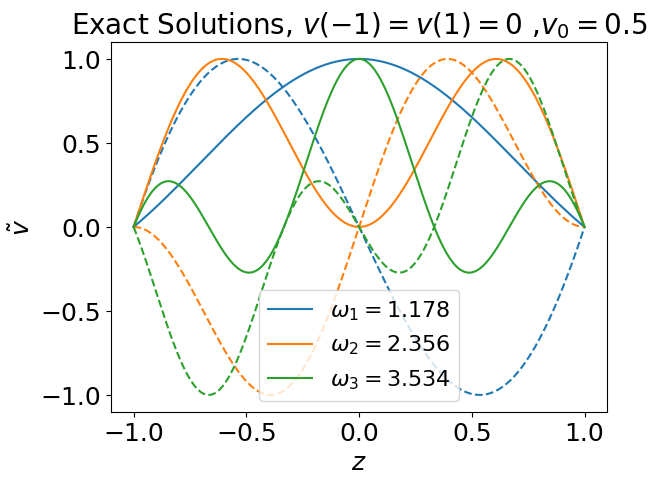
\includegraphics[width=\linewidth]{figures/exact-fixed-fixed-v0=0.5}
		\caption{Subsonic}
	\end{subfigure}%
	\begin{subfigure}{0.5\textwidth}
		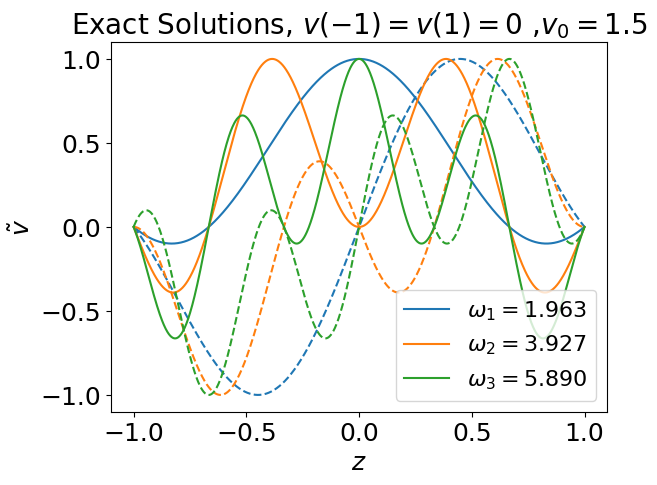
\includegraphics[width=\linewidth]{figures/exact-fixed-fixed-v0=1.5}
		\caption{Supersonic}
	\end{subfigure}
	\caption{The plots show the first three non-zero exact solutions to Eq.~(\ref{eq:constant-v-problem-dirichlet}) for both subsonic and supersonic case. These solutions are stable.}
	\label{fig:exact-v-dirichlet}
\end{figure}

\subsection{Fixed-Open Boundary}
Fixed-Open boundary condition assumes that there are no perturbations at the entrance of the nozzle, and it is free on the exit of the nozzle.

\begin{equation} \label{eq:constant-v-problem-fixed-open}
	\omega^2\tilde{v} + 2i\omega v_0\pdv{\tilde{v}}{z} + (1-v_0^2)\pdv[2]{\tilde{v}}{z} = 0
	\quad
	\tilde{v}(-1) = \pdv{\tilde{v}}{z}\,(1) = 0
\end{equation}

The solution to this problem is similar to Eq.~(\ref{eq:constant-v-solution-dirichlet}), the only difference is the eigenvalues. In this case, the eigenvalues are
\begin{equation}
	\omega_n = (v_0^2 - 1) \left[\frac{n\pi}{2} - \frac{1}{4}i\ln(\frac{v_0-1}{v_0+1})\right], \quad n\in\mathbb{Z}
	\label{eq:eigvals-constant-v-fixed-open}
\end{equation}
The growth rate is independent of the mode number $n$, and it is always $\ln((v_0-1)/(v_0+1))$. It is is positive for any $v_0\neq 1$. Therefore,
\begin{itemize}
	\item If $v_0<1$, then $\Im(\omega)<0$, it's damped oscillation, hence stable.
	\item If $v_0>1$, then $\Im(\omega)>0$, it's unstable.
\end{itemize}

\begin{figure}[htbp]
	\centering
	\begin{subfigure}{0.5\textwidth}
		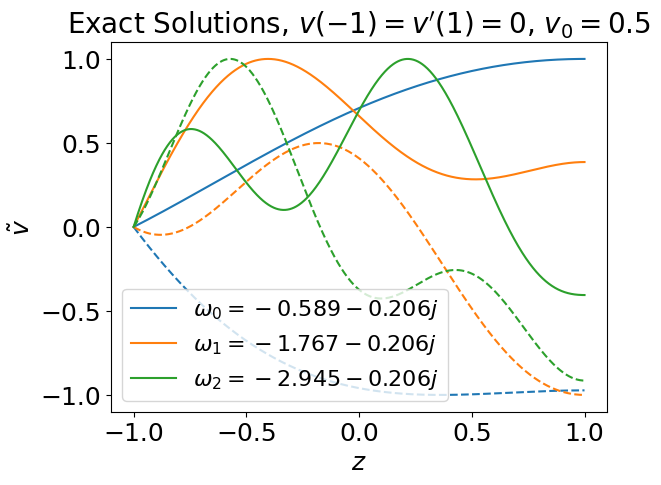
\includegraphics[width=\linewidth]{figures/exact-fixed-open-v0=0.5}
		\caption{Subsonic, stable flow.}
	\end{subfigure}%
	\begin{subfigure}{0.5\textwidth}
		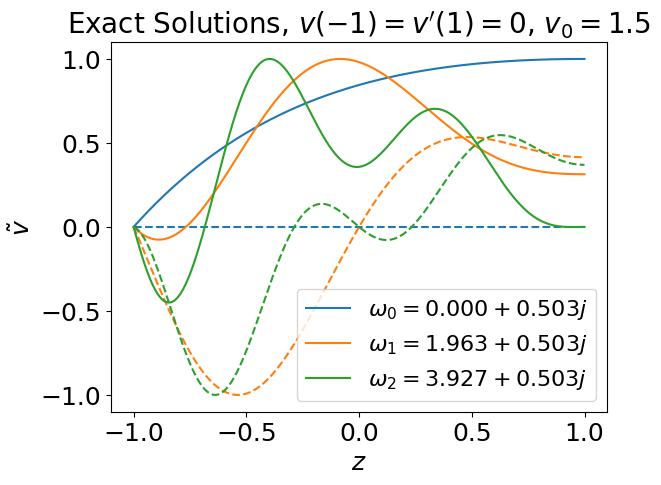
\includegraphics[width=\linewidth]{figures/exact-fixed-open-v0=1.5}
		\caption{Supersonic, unstable flow.}
	\end{subfigure}
	\caption{The plots show the first three exact solutions to Eq.~(\ref{eq:constant-v-problem-fixed-open}) for both subsonic and supersonic case. The flow is stable for subsonic case and unstable for supersonic case.}
	\label{fig:exact-v-fixed-open}
\end{figure}
